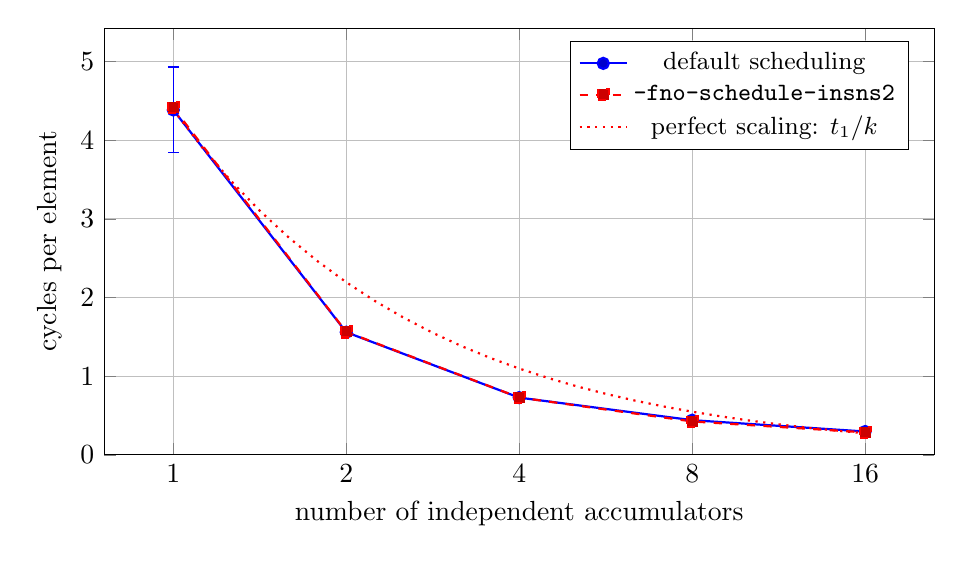
\begin{tikzpicture}
\begin{axis}[width=\textwidth, height=7cm, xmode=log, log basis x=2, xlabel={number of independent accumulators}, ylabel={cycles per element}, grid=major, ymin=0,
  xtick={1,2,4,8,16}, xticklabels={1,2,4,8,16}, legend pos=north east, legend style={font=\small}]
\addplot+[mark=*, thick, error bars/.cd, y dir=both, y explicit] coordinates {(1,4.386) +- (0,0.546) (2,1.560) +- (0,0.058) (4,0.728) +- (0,0.008) (8,0.441) +- (0,0.000) (16,0.297) +- (0,0.006)};
\addlegendentry{default scheduling}
\addplot+[mark=square*, thick, dashed] coordinates {(1,4.413) (2,1.564) (4,0.729) (8,0.425) (16,0.286)};
\addlegendentry{\texttt{-fno-schedule-insns2}}
\addplot[red, dotted, thick, domain=1:16] {4.39/x};
\addlegendentry{perfect scaling: $t_1 / k$}
\end{axis}
\end{tikzpicture}